\section{The goal}
\SectionPage{}

\begin{frame}{The goal}
\emph{Goal}: minimize a cost function \(C\).
\begin{itemize}
    \item<2-> NP-Hard
    \item<3-> Exhaustive search vs heuristics
\end{itemize}
\end{frame}

\begin{frame}{Variational quantum circuits}
Some ideas:
\begin{itemize}
    \item<1-> Quantum circuit as a parametric model;
    \item<2-> Parameters optimized classically. 
\end{itemize}
\end{frame}

\begin{frame}{QAOA}
Steps:
\begin{enumerate}
    \item<1-> define your problem in terms of an Hermitian matrix \(H\), the solution of your problem must coincide with the ground state of \(H\) (eigenvector associated with the minimum valued eigenvalue).
    \begin{itemize}
        \item<2-> we consider only \(H\) diagonal;
        \item<3-> ground state: row (equiv. column) of the computational basis associated to the minimum valued eigenvalue;
        \item<4-> all solutions are from computational basis = retrieve them with certainty.
    \end{itemize}
    \item<5-> build the unitary circuit \(U = e^{iH}\) and make it parametric with a single parameter \(\gamma\): \(U_\gamma = e^{i\gamma H}\);
    \item<6-> build the unitary \(U_\beta\) given by rotating \(\text{Rx}(\beta)\) on any qubit;
    \item<7-> the whole circuit is: \(H^{\otimes n}\) then repeat \(U_{\gamma_i} U_{\beta_i}\) p-times.
\end{enumerate}
\end{frame}


\begin{frame}{QAOA}
\begin{center}
    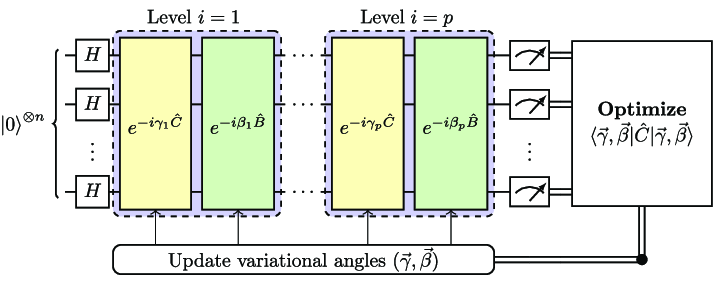
\includegraphics[width=\textwidth]{img/lec6/qaoa.png}
\end{center}
\end{frame}


\begin{frame}{QAOA}
\alert{Note}: no guarantees of performance improvement. 
\end{frame}


\begin{frame}{QAOA}
\alert{Note}: this tutorial is partially inspired by "A tutorial on Quantum Approximate Optimization Algorithm" 

\bigskip\begin{center}\url{youtube.com/watch?v=AOKM9BkweVU}\end{center}

\bigskip Covers much more!
\end{frame}